\chapter{Eidesstattliche Erkl�rung}
Gem�� �\,17,(5) der BPO erkl�re ich an Eides statt, dass ich die vorliegende Arbeit
selbst�ndig angefertigt habe. Ich habe mich keiner fremden Hilfe bedient und keine
anderen, als die angegebenen Quellen und Hilfsmittel benutzt. Alle Stellen, die
w�rtlich oder sinngem�� ver�ffentlichten oder nicht ver�ffentlichten Schriften und
anderen Quellen entnommen sind, habe ich als solche kenntlich gemacht. Diese
Arbeit hat in gleicher oder �hnlicher Form noch keiner Pr�fungsbeh�rde vorgelegen.
\vspace{3\baselineskip}\\
Dortmund, \thedate \hfill \theauthor

\vspace{1cm}
\section*{Erkl�rung}
Mir ist bekannt, dass nach �\,156~StGB bzw. �\,163~StGB eine falsche Versicherung
an Eides Statt bzw. eine fahrl�ssige falsche Versicherung an Eides Statt mit
Freiheitsstrafe bis zu drei Jahren bzw. bis zu einem Jahr oder mit Geldstrafe
bestraft werden kann.
\vspace{3\baselineskip}\\
Dortmund, \thedate \hfill \theauthor

\chapter{About Rover Project}
A4MCAR is not the only demonstrator for APP4MC. In the Rover project, investigation of APP4MC's effectiveness is done by using a more stable POSIX thread-based platform using only C++ language. The developments for the Rover has lots of synergies with Eclipse's PolarSys project.  APP4MC Rover also requires a lot of effort towards Cloud \& IoT based developments such as implementing a bidirectional data communication with an Eclipse Hono cloud instance.

The author of this report is also engaged with tackling tasks in the Rover project. Ensuring schedulable and traceable thread-based software architecture is one of the most crucial challanges in the Rover project. Rover is developed with a much more advanced web interface that can display sensor information, utilization information, control the Rover, and switch between driving modes such as manual driving, Adaptive Cruise Control, and Parking. Some figures are given with the Figure \ref{fig:rover} that depict the progress in the Rover project.

Rover project is being developed in IDiAL Institute of University of Applied Sciences and Arts Dortmund and it is accessible from the following link:

${https://git.eclipse.org/r/plugins/gitiles/app4mc/org.eclipse.app4mc.examples/+/master}$

\begin{figure}[!ht]
	\centering
	\captionsetup{justification=centering}
	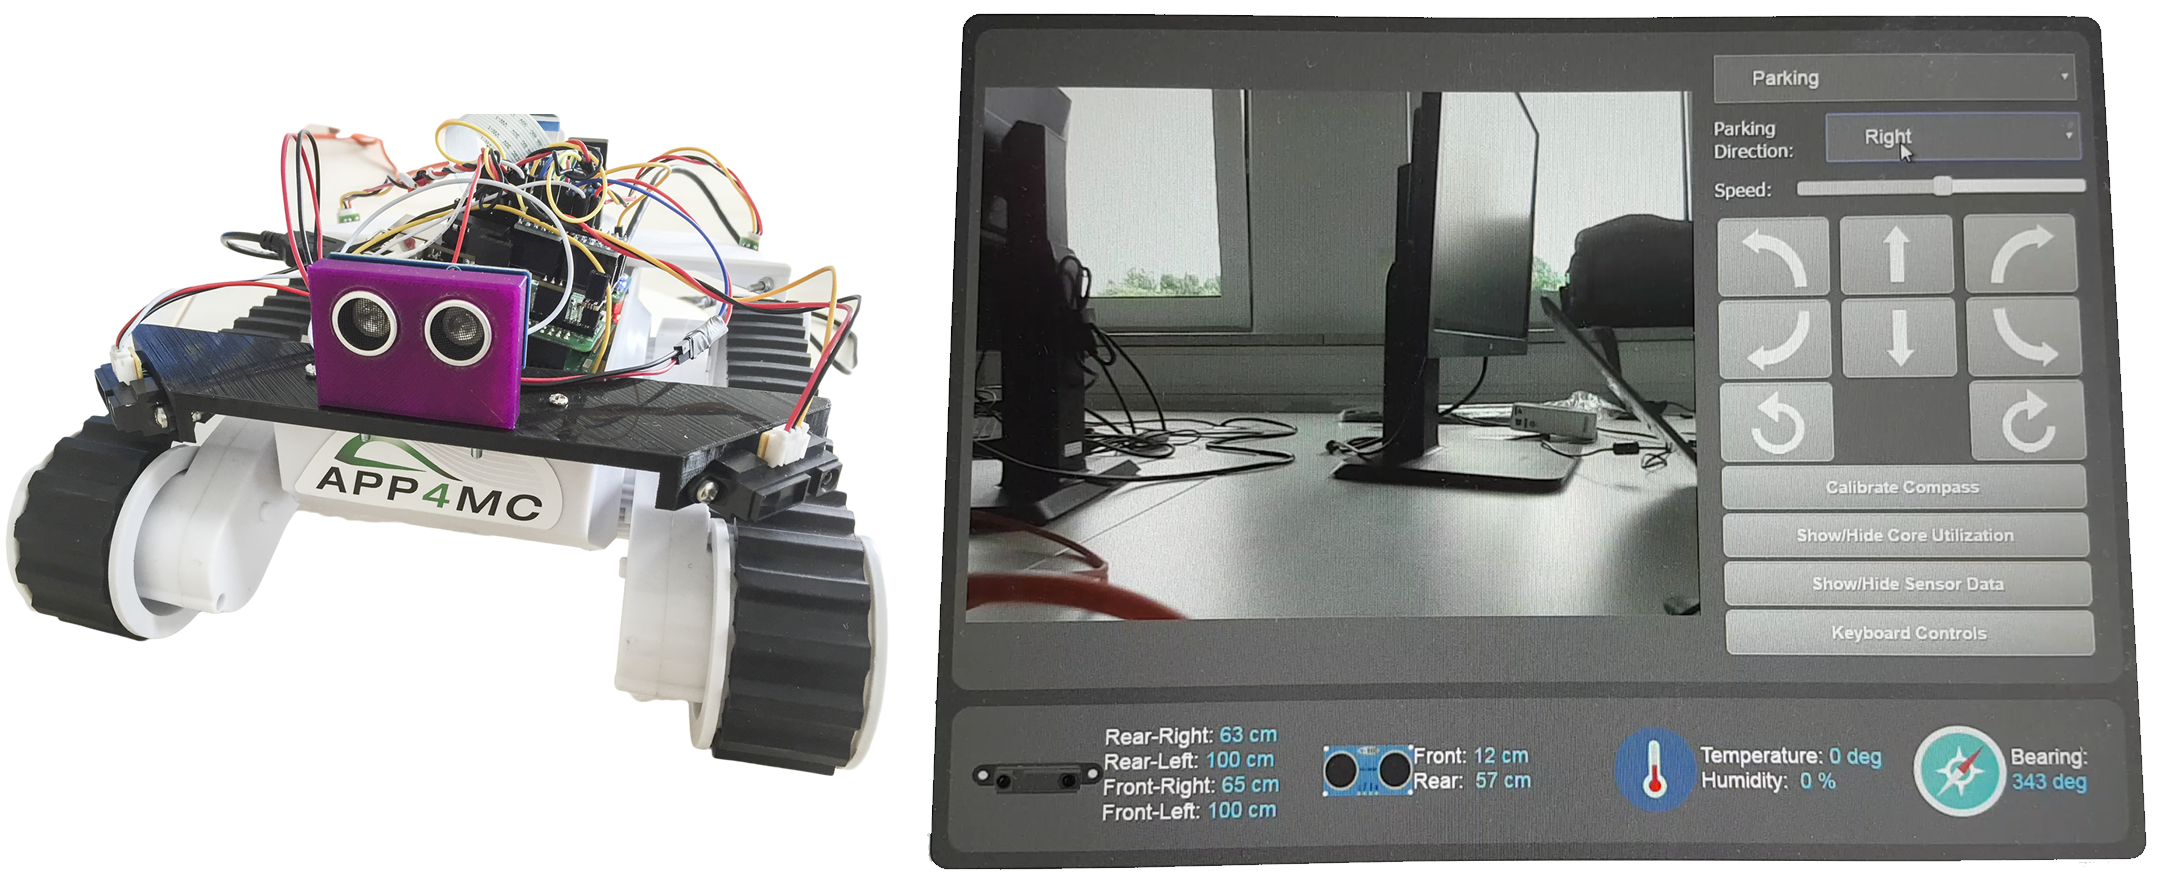
\includegraphics[width=\textwidth]{content/images/rover.png}
	\caption{Rover project and its web interface}
	\label{fig:rover}
\end{figure}
